\section{Software description}
\label{sec:SoftwareDescription}

The proposed software architecture is engineered as a decoupled, modular system designed to bridge conversational natural language processing, spatial search engine indexing, and interactive web mapping. The design prioritizes strict separation of concerns, defensive programming against LLM hallucinations, and immediate cartographic visual feedback.

\subsection{Software Architecture Overview}
\label{subsec:SoftwareArchitecture}

The architecture is structured around four decoupled execution stages, as illustrated in the workflow diagram in Figure~\ref{fig:arch}.

\begin{figure}[h!]
\centering
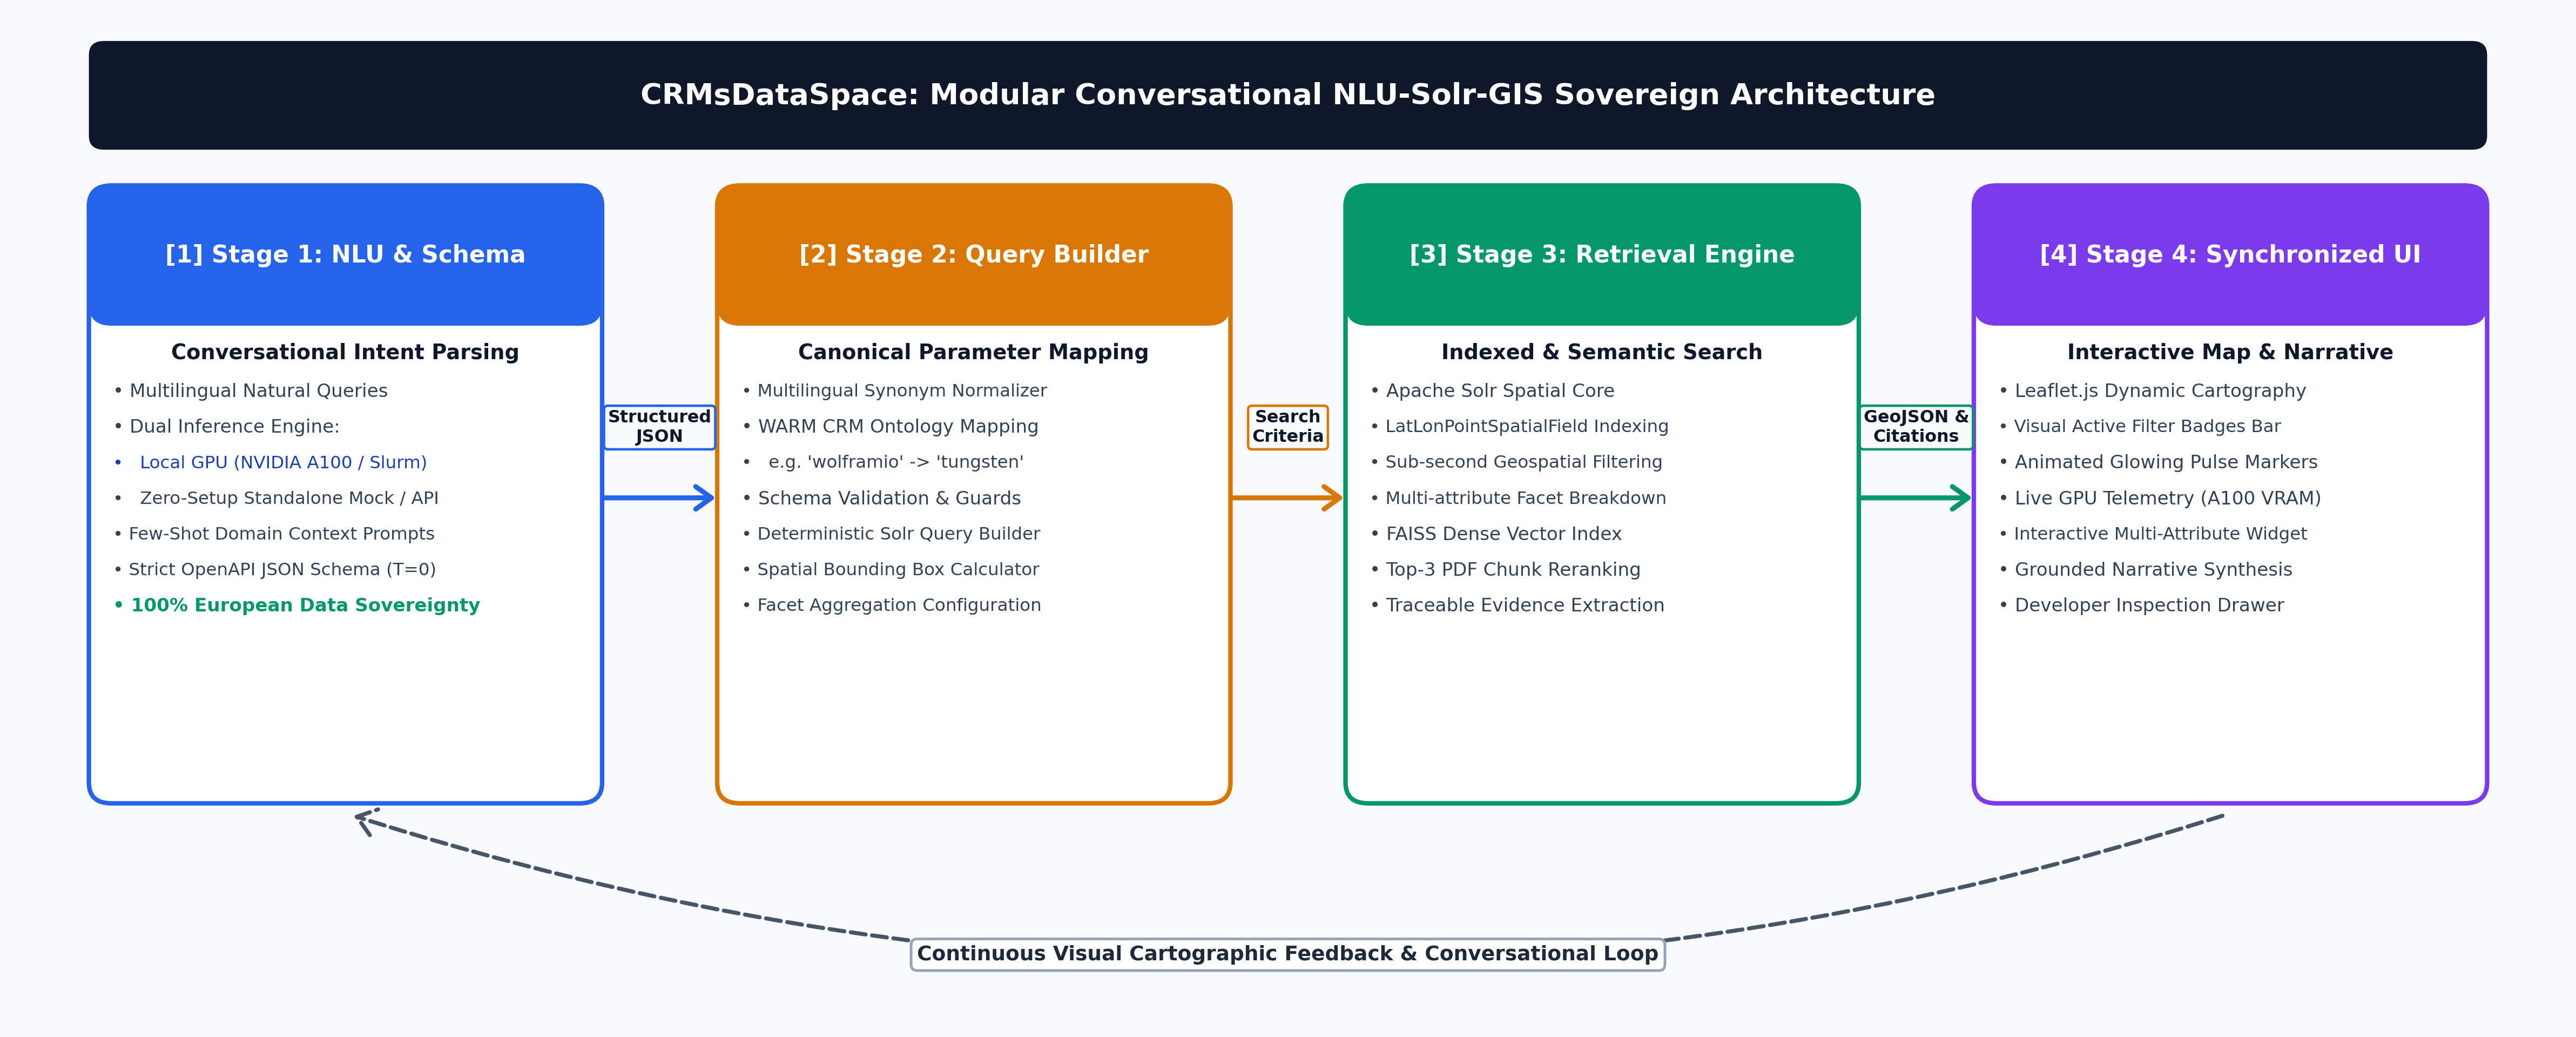
\includegraphics[width=0.98\textwidth]{architecture_diagram.png}
\caption{Overall decoupled software pipeline architecture combining conversational NLU intent parsing, query generation, spatial search engine retrieval, and dynamic GIS web map synchronization.}
\label{fig:arch}
\end{figure}

The functional workflow operates through four decoupled layers:

\begin{enumerate}
    \item \textbf{Stage 1: Conversational NLU \& Schema Enforcement}: The user submits a free-text spatial query $Q$ through the web interface. Rather than permitting unconstrained text generation, the query is processed by a dual-variant NLU parser that combines Few-Shot contextual exemplars with a strict OpenAPI JSON Schema evaluated under greedy decoding ($T = 0.0$)~\cite{willard2023outlines, gemini2024}. This contract guarantees that the extracted payload strictly adheres to pre-defined intent types and entity slots, completely eliminating database schema hallucinations (Figure~\ref{fig:comp1}).
    
    \begin{figure}[h!]
    \centering
    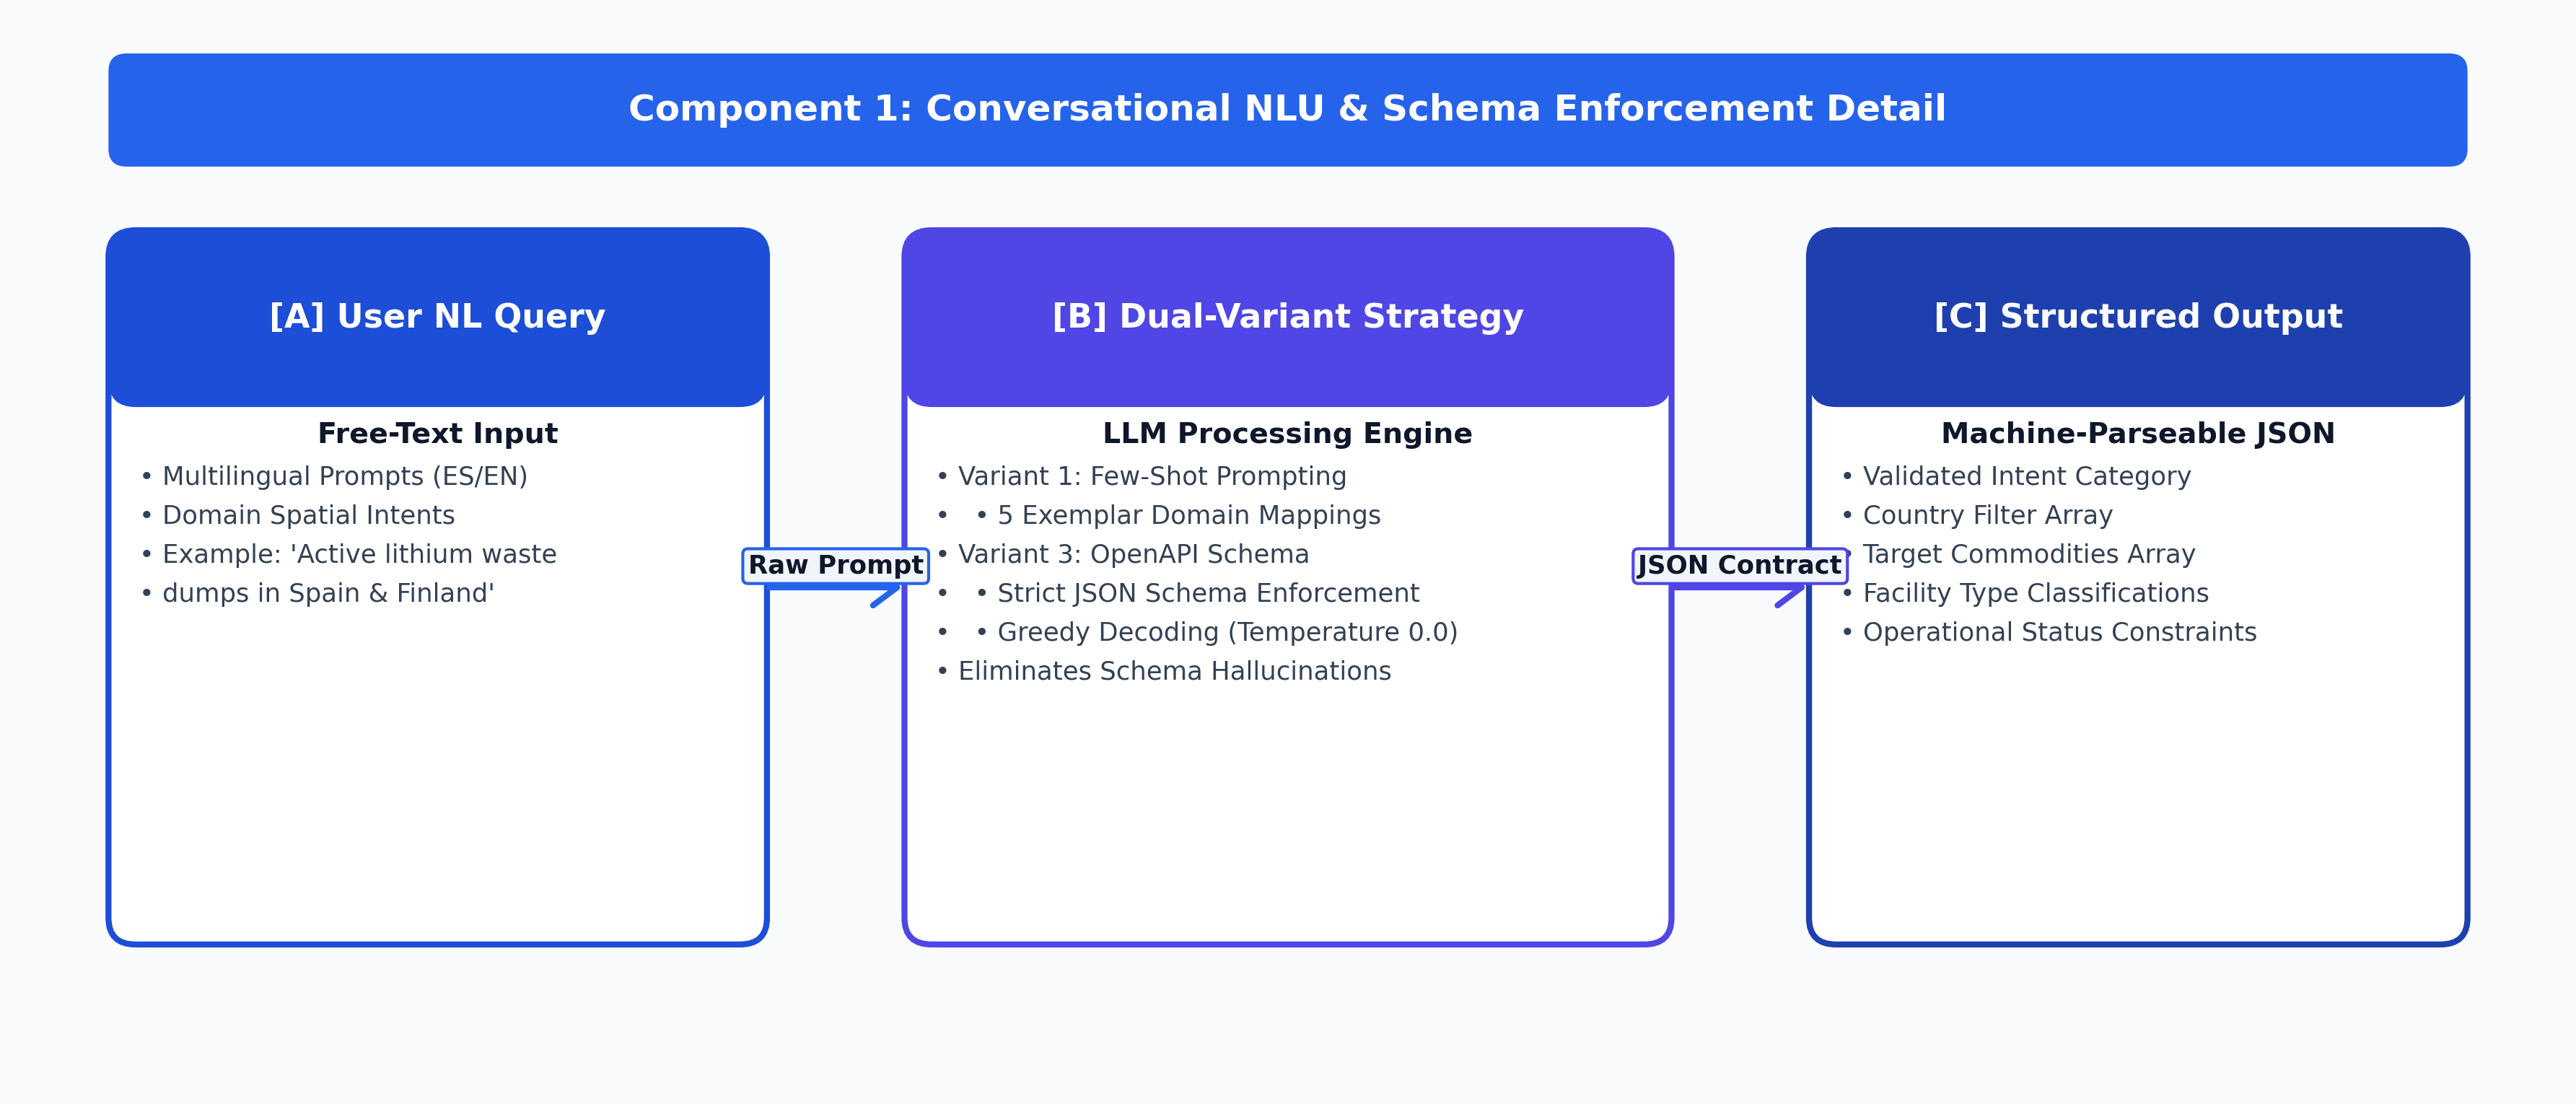
\includegraphics[width=0.90\textwidth]{component1_nlu_schema.png}
    \caption{Workflow of Stage 1: Conversational NLU Intent Parsing with dual-variant Few-Shot prompting and OpenAPI JSON Schema enforcement.}
    \label{fig:comp1}
    \end{figure}

    \item \textbf{Stage 2: Pluggable Domain Normalization \& Search Query Generation}: Extracted entity values frequently contain informal expressions, regional language synonyms, or chemical element symbols. Component~2 routes these values through a pluggable domain thesaurus that normalizes terms into canonical vocabularies aligned with standard reporting taxonomies~\cite{ballatore2014vocabulary}. A schema validator verifies structural integrity before constructing disjunctive and conjunctive Boolean search filter arrays for Apache Solr (Figure~\ref{fig:comp2}).

    \begin{figure}[h!]
    \centering
    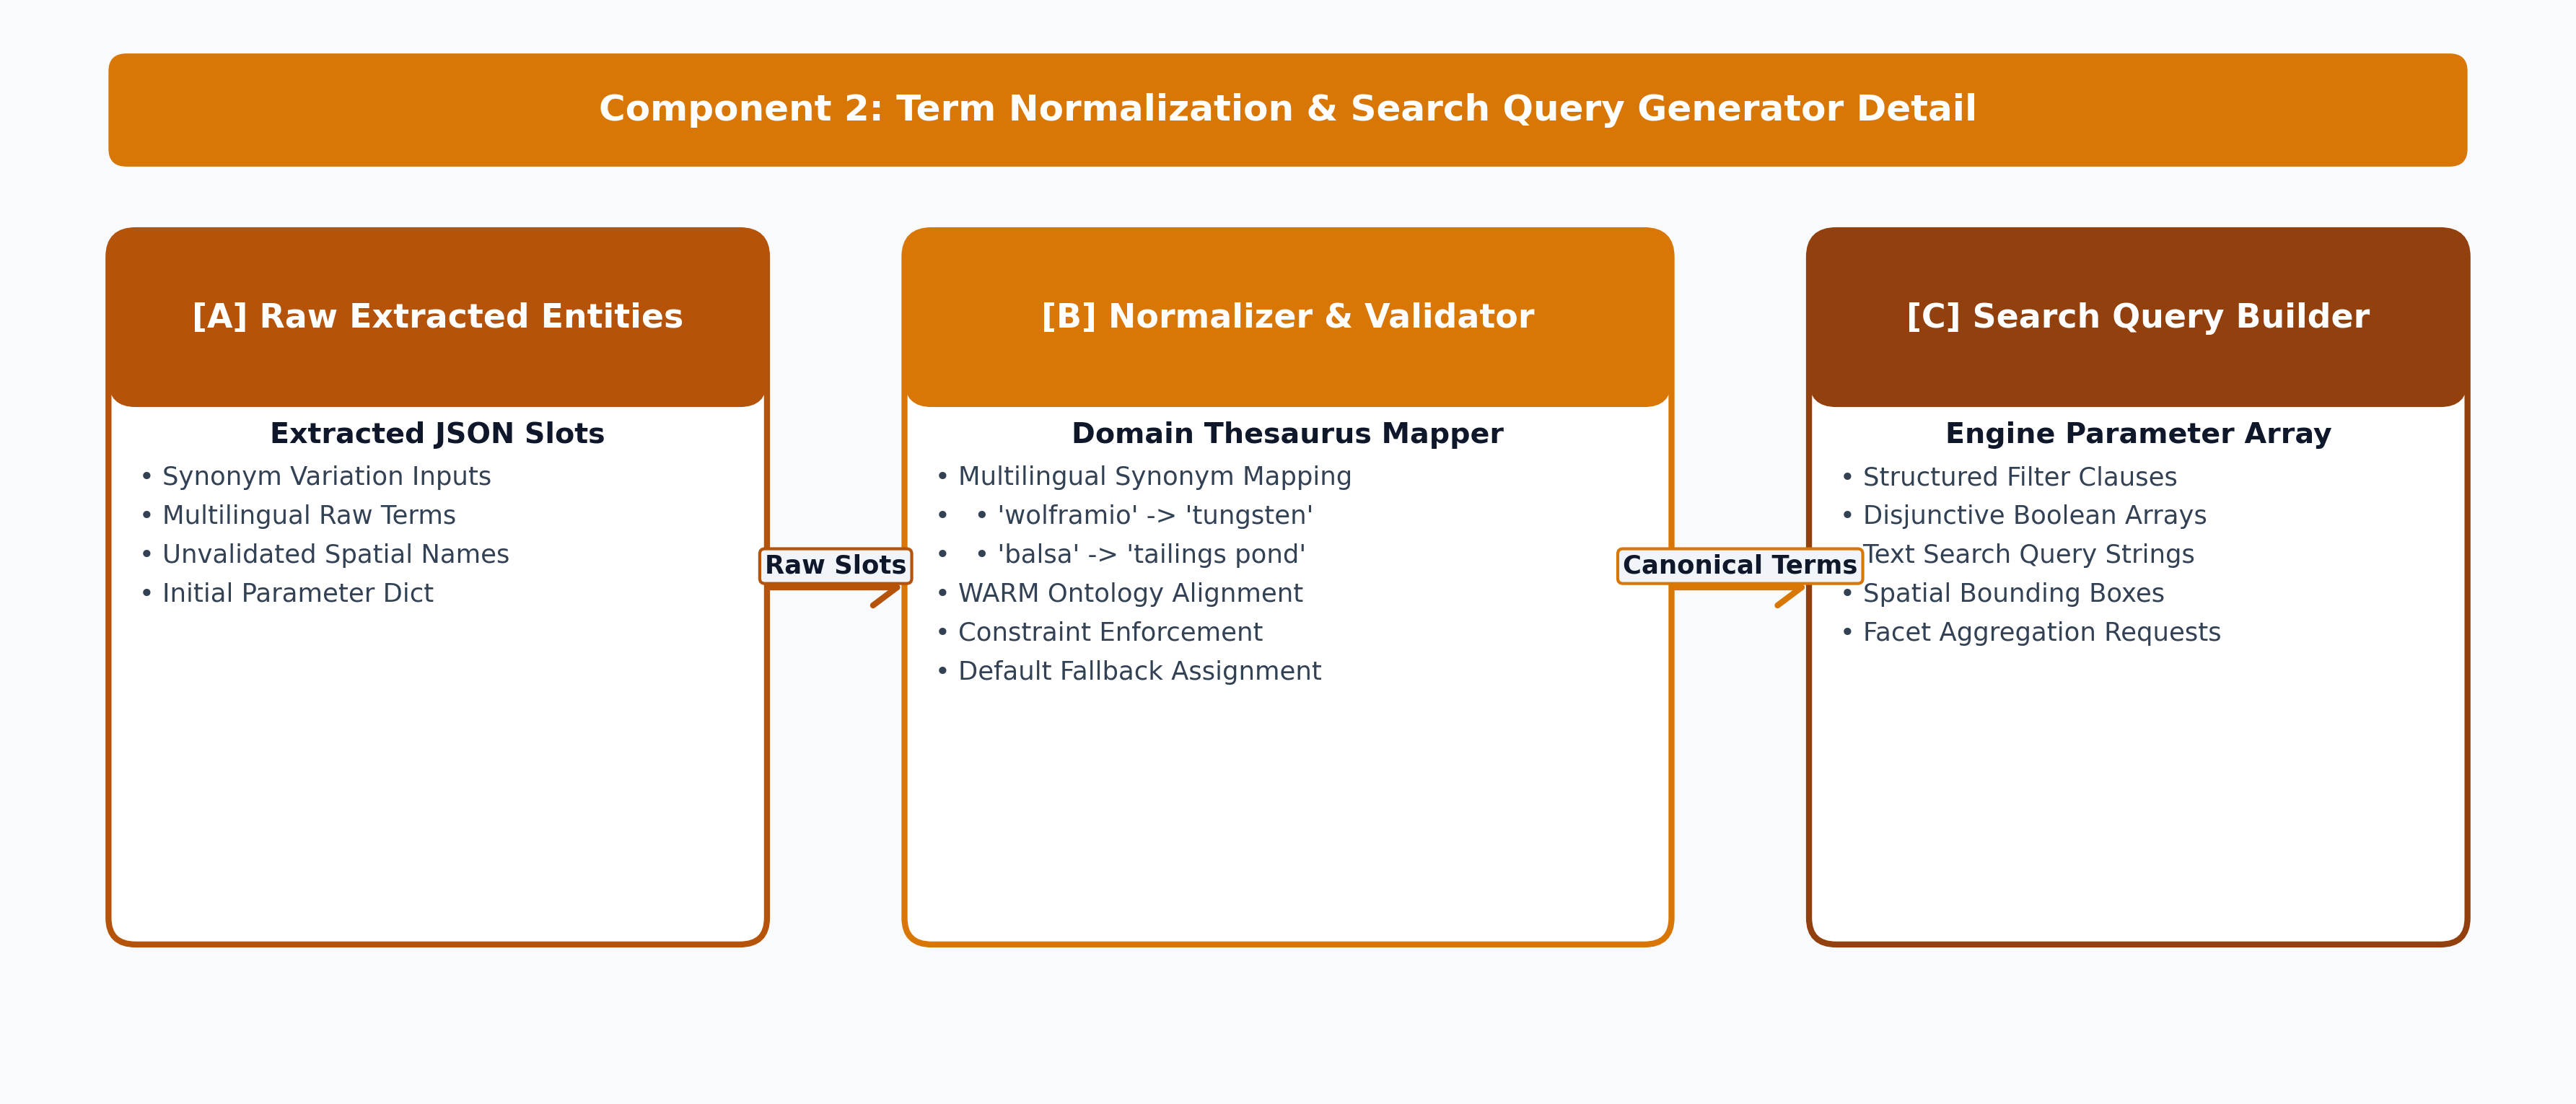
\includegraphics[width=0.90\textwidth]{component2_query_builder.png}
    \caption{Workflow of Stage 2: Multilingual Domain Term Normalization, Validation, and Solr Filter Query Generation.}
    \label{fig:comp2}
    \end{figure}

    \item \textbf{Stage 3: Spatial Search Engine Indexing \& Vector Evidence Retrieval}: The generated filter queries execute against an Apache Solr spatial engine~\cite{solr2020}. In production data spaces such as CRMsDataSpace, the retrieval layer interfaces with a distributed \textbf{SolrCloud} cluster coordinated via Apache ZooKeeper, providing high availability, fault-tolerant horizontal sharding across heterogeneous regional nodes, and automated replication for continent-wide extractive inventories. The software architecture is completely agnostic to the underlying deployment topology: the query generator produces standard Lucene filter parameters (\texttt{q}, \texttt{fq}, and faceting directives over standard HTTP REST endpoints) that interface identically with distributed SolrCloud collections, single-node Solr standalone cores, or the embedded zero-setup standalone mock engine via environment variable configuration (\texttt{SOLR\_URL}). Solr evaluates geospatial constraints using spatial indexing fields (such as \texttt{LatLonPointSpatialField} and bounding box filters) and computes live multi-dimensional facet distributions~\cite{solr2020, manning2008information}. In parallel, when the query requests unstructured technical or regulatory evidence, a dense vector index (FAISS)~\cite{johnson2019billion, lewis2020retrieval} performs similarity retrieval over document chunks, applying an information-density reranker to select top-scoring citation snippets (Figure~\ref{fig:comp3}).

    \begin{figure}[h!]
    \centering
    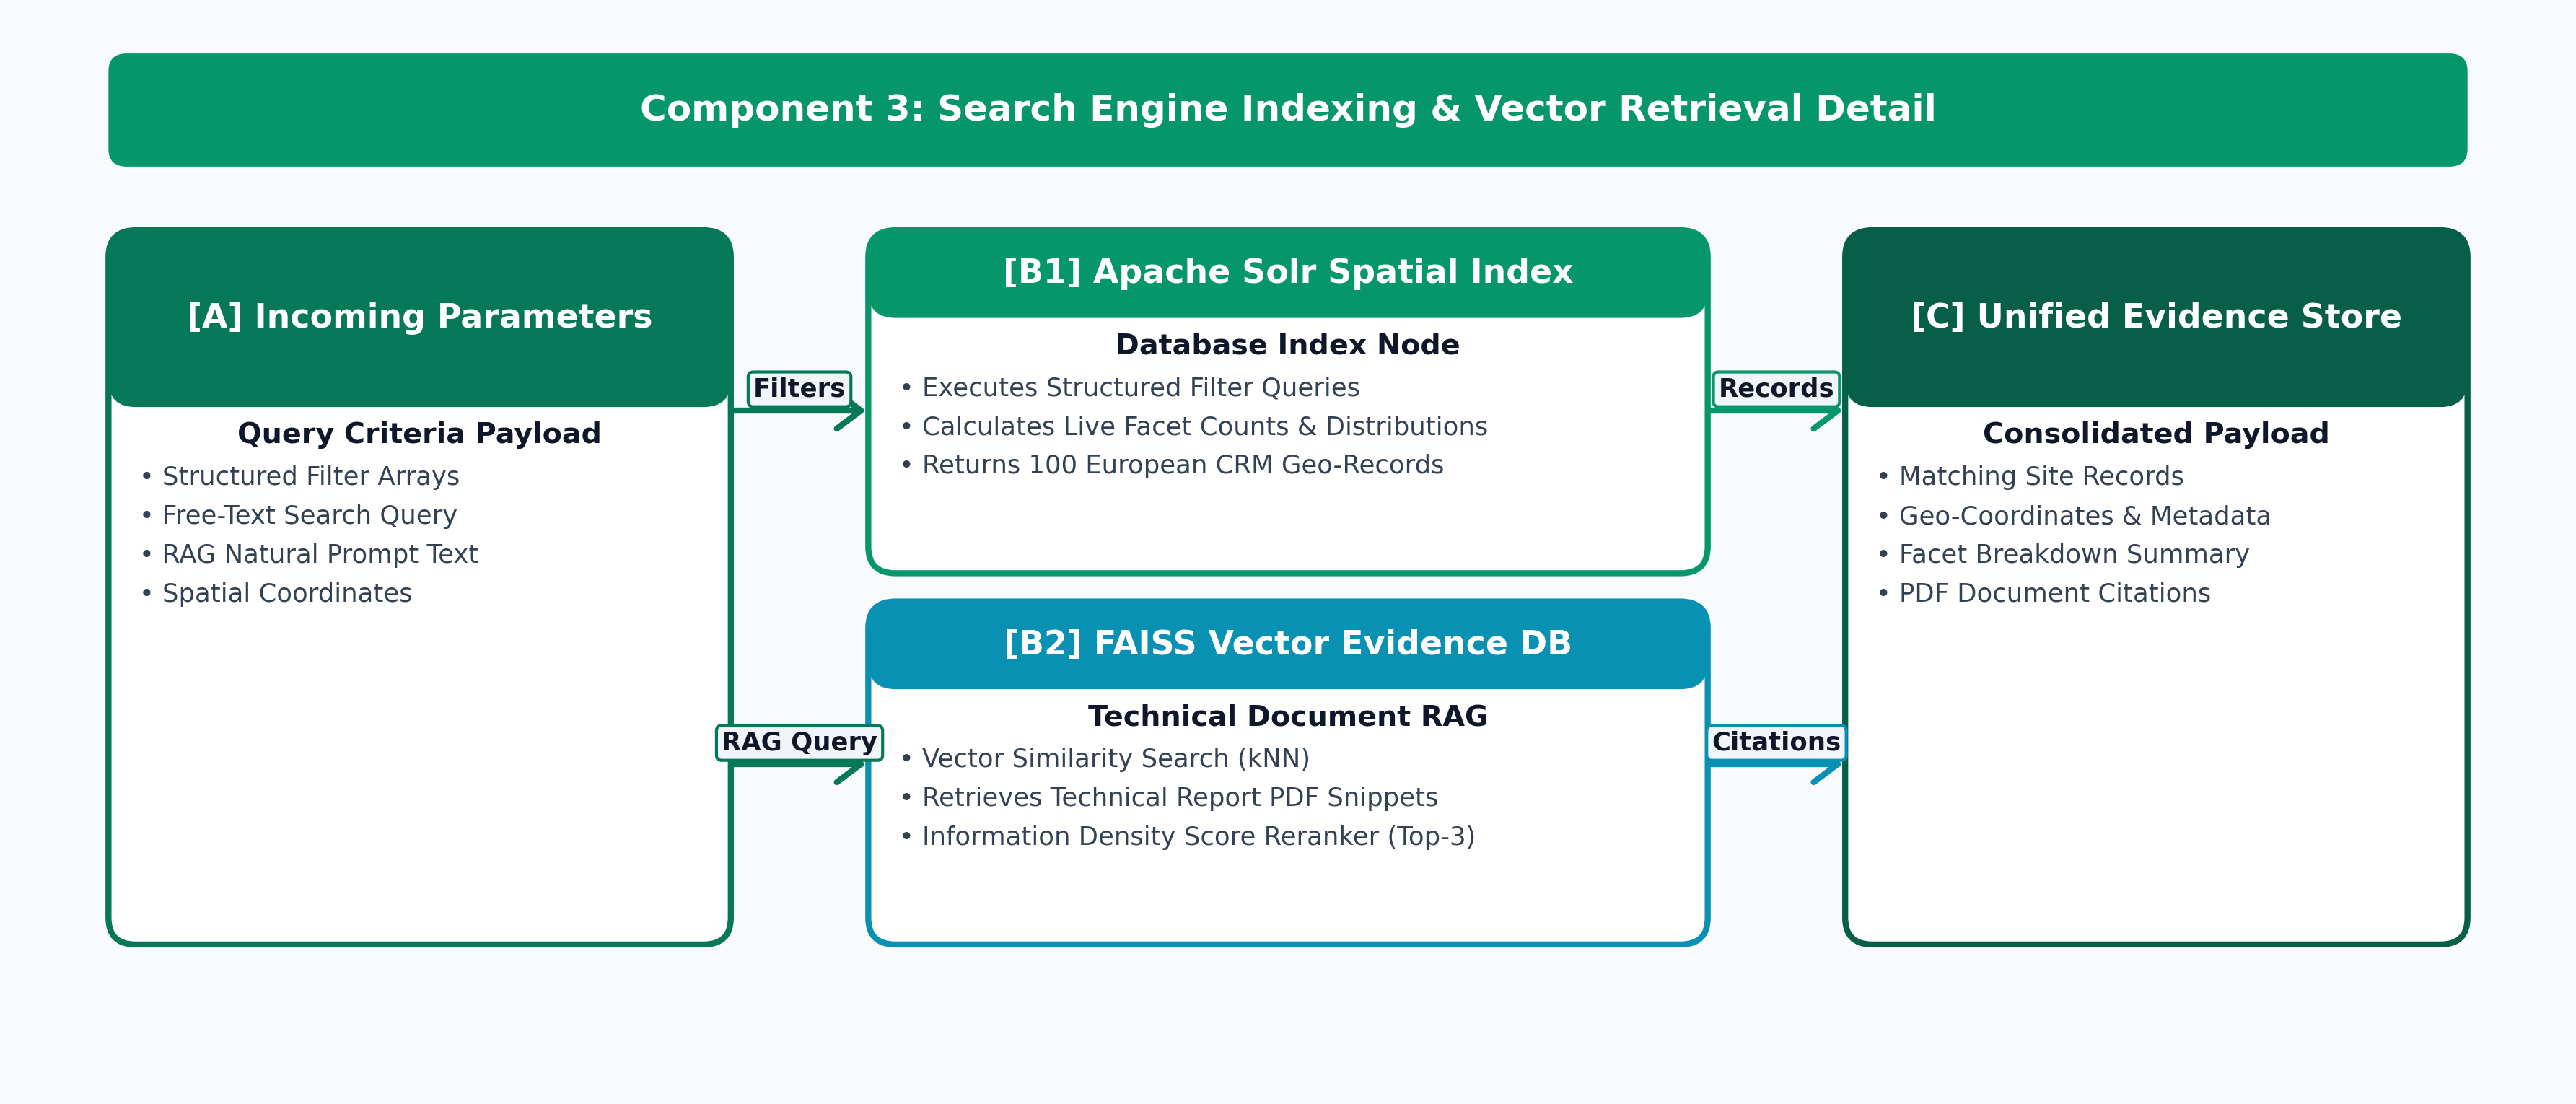
\includegraphics[width=0.90\textwidth]{component3_search_rag.png}
    \caption{Workflow of Stage 3: Dual Spatial Search Engine (Apache Solr) and Technical Document Vector Retrieval (FAISS).}
    \label{fig:comp3}
    \end{figure}

    \item \textbf{Stage 4: Dynamic GIS Map \& Conversational Web Dashboard}: The client web application, built with Leaflet.js~\cite{leaflet2023} and TailwindCSS, receives the consolidated spatial records, facet statistics, and textual evidence. As illustrated in Figure~\ref{fig:comp4}, the interface integrates real-time GPU VRAM telemetry (A), an active visual filter sub-bar (B), dynamic cartography with animated glowing pulse rings (C), a grounded conversational chat assistant with traceable document citations (D), and a slide-out developer inspection drawer (E) providing full transparency into intermediate JSON artifacts and executed Solr parameters.

    \begin{figure*}[t!]
    \centering
    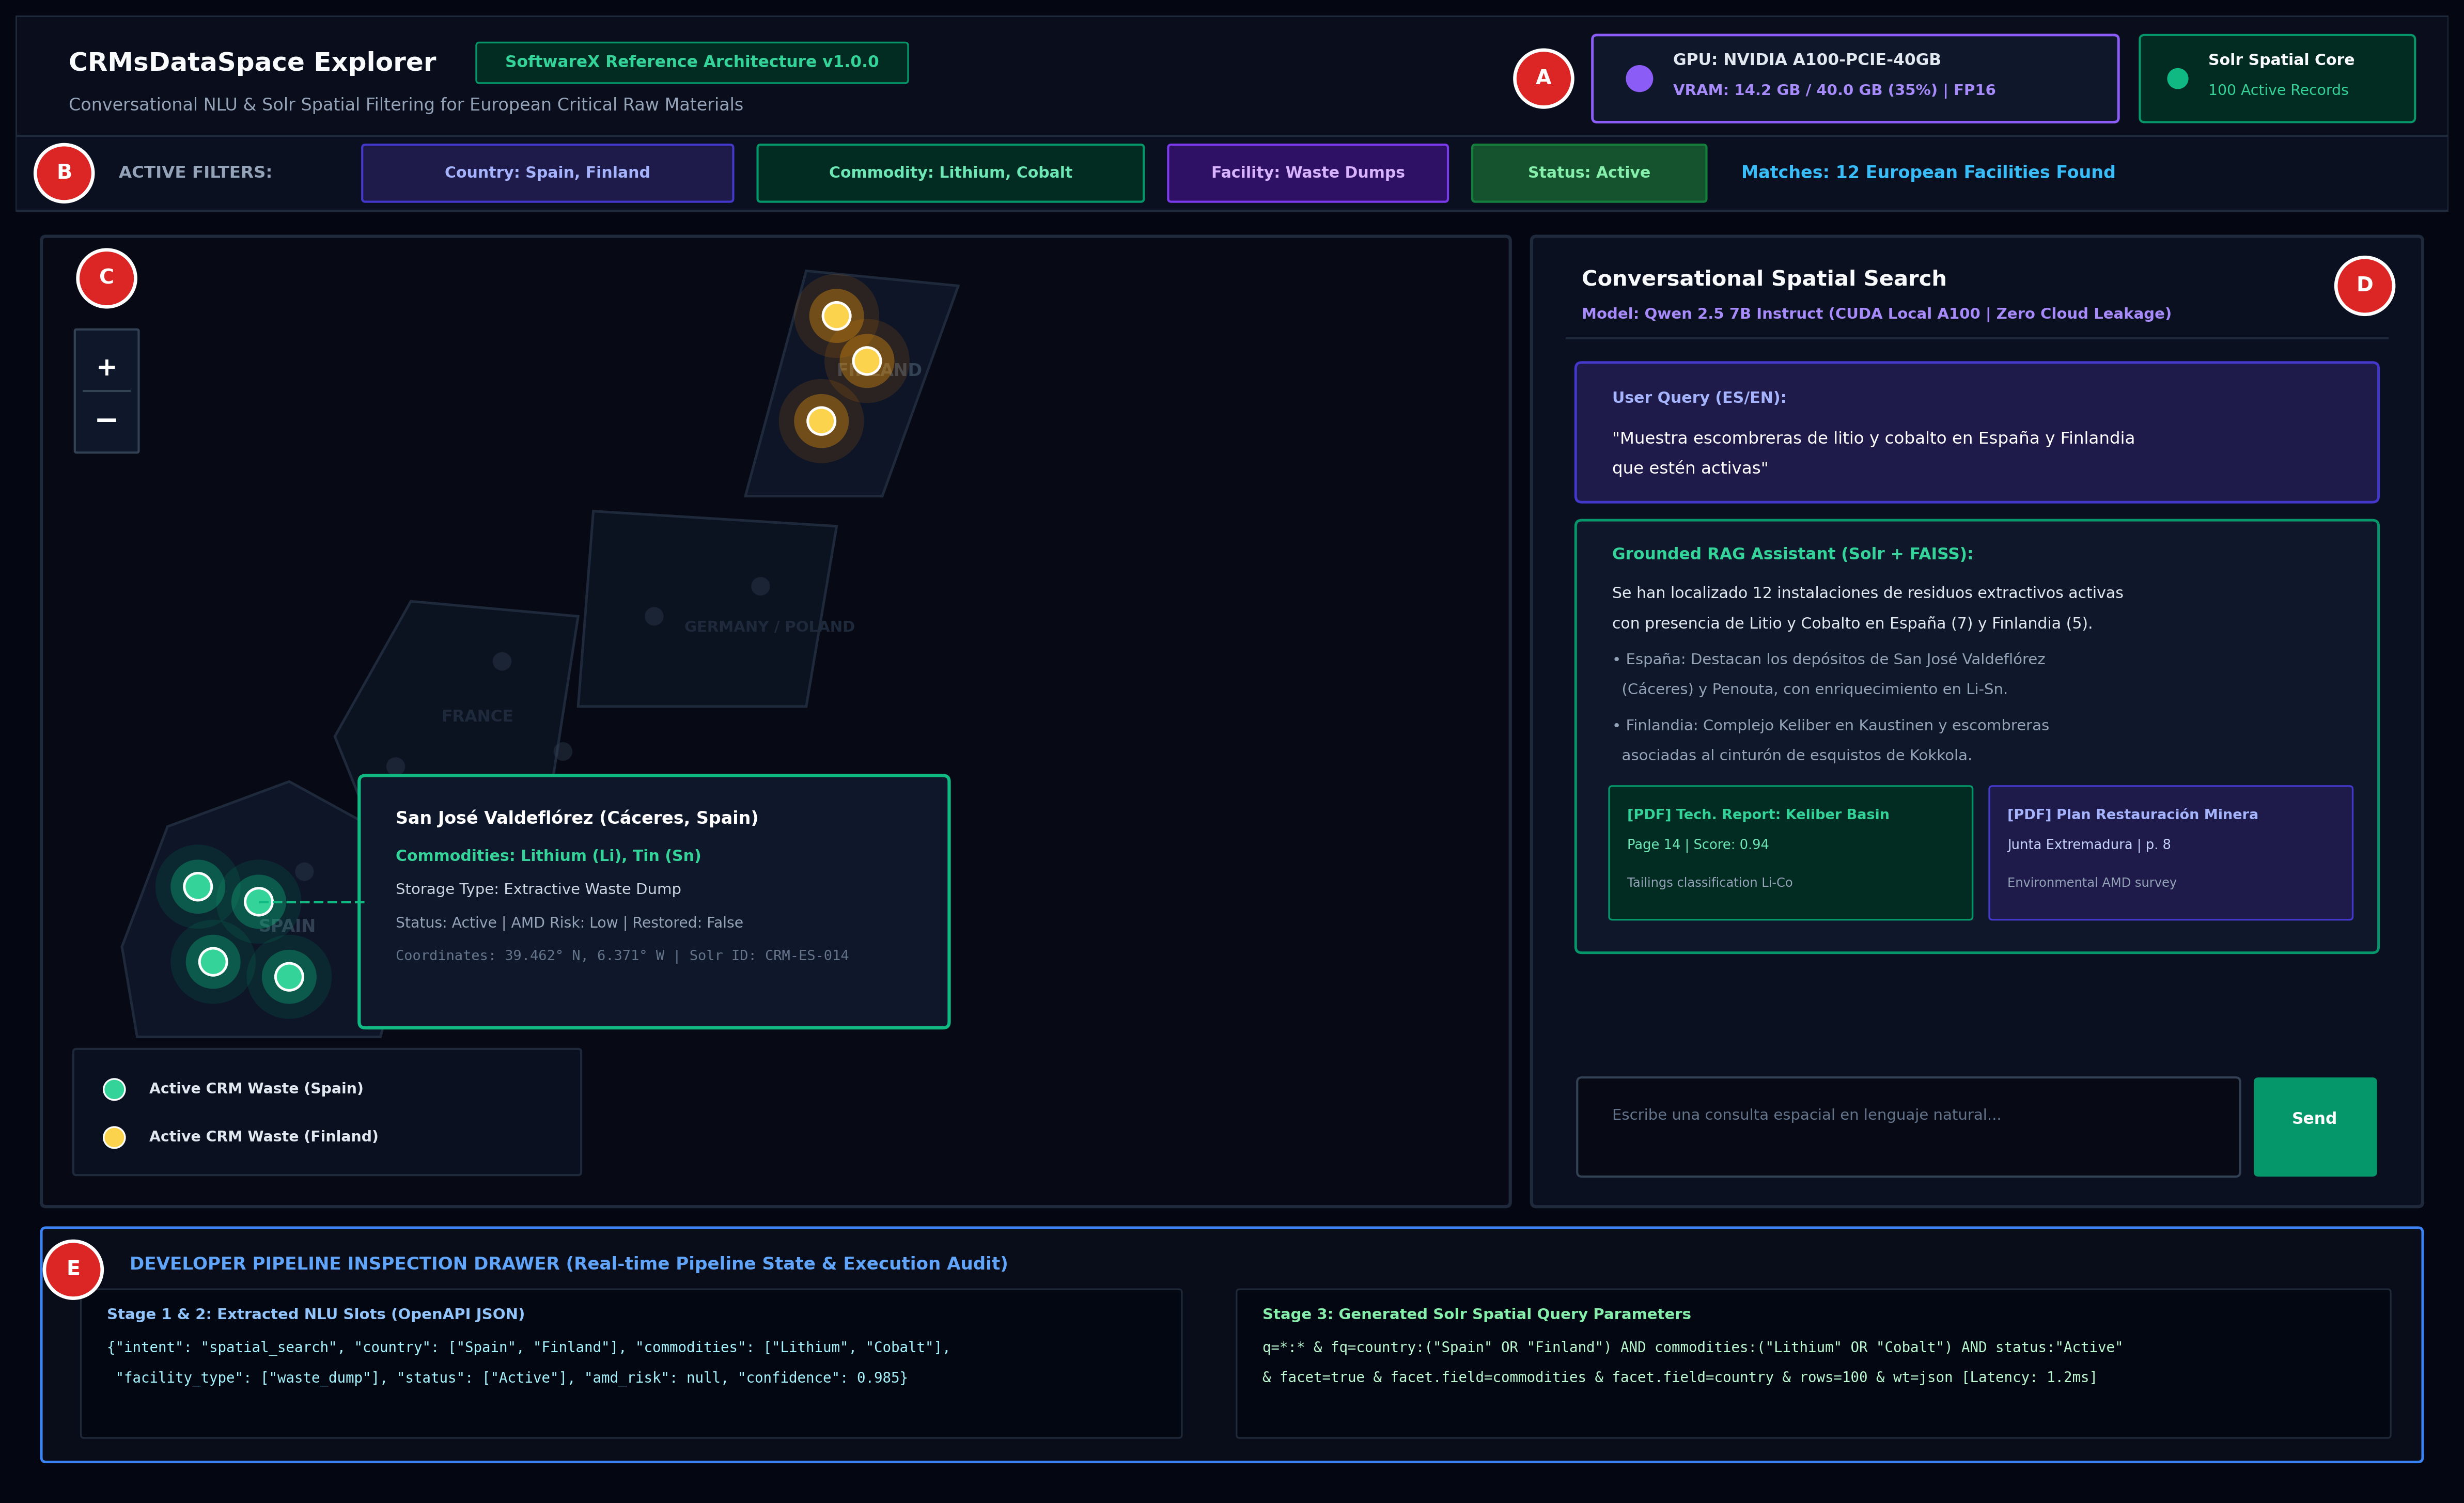
\includegraphics[width=\textwidth]{component4_gis_ui.png}
    \caption{Annotated operational interface of the CRMsDataSpace web demonstrator: (A)~Real-time GPU VRAM telemetry badge monitoring on-premises NVIDIA A100 inference; (B)~Dynamic active visual filter sub-bar translating conversational criteria into filter pills; (C)~Interactive Leaflet.js GIS map with animated glowing pulse markers on matching European CRM waste facilities and popup metadata cards; (D)~Grounded conversational chat synthesizing responses with traceable PDF technical evidence cards; (E)~Slide-out developer inspection drawer for live auditing of intermediate OpenAPI JSON extractions and Solr spatial filter parameters.}
    \label{fig:comp4}
    \end{figure*}
\end{enumerate}

\subsection{Software Functionalities}
\label{subsec:SoftwareFunctionalities}

The software architecture delivers the following general-purpose capabilities:

\begin{itemize}
    \item \textbf{Multi-Criteria Natural Language Filtering}: Users can formulate complex queries combining geographic boundaries, domain commodities/categories, physical facility types, and operational/environmental conditions.
    \item \textbf{Dynamic GIS Visual Synchronization \& Multi-Select Attribute Widget}: Extracted search criteria are converted into interactive visual badges on the map header and automatically populate a floating multi-selection attribute panel. Users can toggle multiple jurisdictions (e.g., cross-border queries spanning Spain and Portugal) or commodities manually with immediate two-way state synchronization. The map viewport dynamically focuses on the filtered cluster, triggering animated pulsing markers on matching sites while dimming non-matching locations to guide visual exploration.
    \item \textbf{Dual-Topology Search Integration (SolrCloud \& Standalone Mock)}: Designed for seamless transition from research validation to enterprise deployment, the architecture interfaces directly with distributed \textbf{SolrCloud} clusters (leveraging ZooKeeper orchestration, sharding, and replication) via standard HTTP REST endpoints, while offering an automated fallback to an embedded zero-setup standalone mock engine with 100 georeferenced synthetic European CRM sites for dependency-free reviewer reproducibility.
    \item \textbf{Grounded Evidence and Anti-Hallucination Guard}: If zero records match a spatial query or if requested technical documentation is absent, the system executes an early exit guard returning a standard traceability message (\textit{``Information not available in data space''}), preventing the generation of fabricated values or fictitious coordinates.
    \item \textbf{Interactive Pipeline Inspection Drawer}: A slide-out developer panel allows researchers and engineers to inspect the exact intermediate JSON artifacts, extracted slots, normalized entities, and executed Solr filter parameters in real time.
    \item \textbf{On-Premises Local GPU Execution and Data Sovereignty}: Native execution of open-source foundation models on private GPU clusters, ensuring that zero data leaves local infrastructure while eliminating commercial API key dependencies.
\end{itemize}

\subsection{On-Premises Local GPU Inference and European Data Sovereignty}
\label{subsec:DataSovereignty}

A critical requirement in strategic domains such as the European Critical Raw Materials Data Space is preserving \textit{data sovereignty} and confidentiality under Regulation (EU) 2024/1252~\cite{european2024crma, ballatore2014vocabulary}. Routing spatial queries through commercial cloud APIs introduces severe risks of confidential data leakage, regulatory non-compliance under GAIA-X air-gapped mandates, and unpredictable subscription overheads.

To guarantee complete sovereignty, the architecture natively supports on-premises execution of open-weight foundation models directly on private GPU clusters. It integrates four open-source architectures spanning complementary scales: \textbf{Qwen 2.5 7B Instruct} (high-capacity multilingual slot extraction), \textbf{DeepSeek R1 Distill Qwen 7B} (reasoning distillation), \textbf{Phi-3 Mini 4K Instruct} (compact high-throughput inference), and \textbf{Llama 3.2 3B Instruct} (lightweight execution for departmental GPUs).

The local inference subsystem is implemented using PyTorch, Hugging Face Transformers, and CUDA~12 with FP16 half-precision tensor execution. To guarantee that memory consumption remains strictly contained on institutional GPU infrastructure, the runtime incorporates an automated VRAM memory lifecycle manager. When switching between foundation models, the engine invokes an explicit memory eviction cycle, reclaiming tensor allocations down to 0.0~GB. This eliminates memory fragmentation and allows a single institutional GPU to host different model architectures sequentially without system restarts. A dedicated REST telemetry endpoint continuously streams allocated VRAM and memory utilization to the Leaflet dashboard, providing real-time auditing of computational resources.

\subsection{Deterministic Query Formalization and Parameter Mapping}
\label{subsec:QueryFormalization}

To guarantee absolute interoperability between conversational NLU and structured spatial search, query transformation is formalized as a deterministic mapping function. Let a user query be denoted by $Q$. The NLU parsing step maps $Q$ into an operational intent class $I$ (such as spatial search, multi-criteria filtering, hybrid queries, or domain guidance) and an entity slot dictionary $S$:
\begin{equation}
    (I, S) = \mathcal{M}_{\text{LLM}}(Q \mid \mathcal{P}_{\text{few-shot}}, \mathcal{S}_{\text{OpenAPI}})
\end{equation}
where $\mathcal{S}_{\text{OpenAPI}}$ denotes the strict JSON Schema enforced during decoding. The schema defines the permissible extraction space across six dimensions: operational intent classes (spatial search, attribute filtering, hybrid QA, domain help), administrative jurisdictions (countries, regions), mineral commodities (CRMs), facility typologies (waste dumps, tailings ponds), operational lifecycles (active, closed), and environmental restoration status.

The extracted slots are normalized through the domain thesaurus $\mathcal{T}$:
\begin{equation}
    S_{\text{canonical}} = \mathcal{T}(S) = \{k: [c(v) \mid v \in S[k]] \quad \forall k \in \text{dom}(S)\}
\end{equation}
Once validated, the normalized slots $S_{\text{canonical}}$ are transformed into an array of Apache Solr filter queries $F_q = \{f_1, f_2, \dots, f_m\}$, where each non-empty attribute array is mapped to a disjunctive constraint joined by Boolean OR, and all active dimensions are combined via Boolean AND. For example, an extraction specifying target countries and commodities translates into structured spatial constraints combined with any active environmental remediation criteria. This parameter mapping completely decouples natural language phrasing from the physical database schema, rendering the software immune to prompt injection attacks or unexpected schema drift. The complete declarative schema definitions and translation logic are available in the project repository.

\subsection{Scalability and Performance Analysis}
\label{subsec:ScalabilityPerformance}

To assess the operational viability of the architecture across computational environments, we evaluated pipeline stage latency across both zero-setup Standalone Mock execution and sovereign On-Premises GPU inference on an NVIDIA A100 testbed.

\begin{table}[h!]
\centering
\small
\setlength{\tabcolsep}{5pt}
\caption{Architectural pipeline latency breakdown across execution modes evaluated over 100 georeferenced European sites.}
\label{tab:performance_metrics}
\begin{tabularx}{0.92\linewidth}{>{\raggedright\arraybackslash}X>{\centering\arraybackslash}p{2.0cm}>{\centering\arraybackslash}p{1.6cm}>{\centering\arraybackslash}p{1.6cm}>{\centering\arraybackslash}p{2.0cm}}
\toprule
\textbf{Execution Mode} & \textbf{NLU Lat.} & \textbf{Search} & \textbf{GIS Sync} & \textbf{Total Latency} \\
\midrule
Standalone Mock (CPU) & 0.4 ms & 1.2 ms & 14.5 ms & \textbf{16.1 ms} \\
Local GPU (Qwen 2.5 7B) & 1,805.5 ms & 1.4 ms & 15.0 ms & \textbf{1,821.9 ms} \\
Local GPU (Llama 3.2 3B) & 1,910.7 ms & 1.4 ms & 14.8 ms & \textbf{1,926.9 ms} \\
\bottomrule
\end{tabularx}
\end{table}

As documented in Table~\ref{tab:performance_metrics}, Standalone Mock Mode achieves near-instantaneous execution ($\sim$16.1~ms end-to-end), making it ideal for continuous integration, regression testing, and rapid reviewer verification. Under on-premises local GPU execution, inference completes in under 1.9~seconds with zero external cloud dependencies, while spatial search indexing and Leaflet cartographic rendering execute in under 17~ms. In the browser client, the Leaflet engine effortlessly renders 100+ animated pulsed SVG markers at 60 frames per second with a memory footprint under 35~MB.

\subsection{Execution Safety, Input Sanitization, and Fault Tolerance}
\label{subsec:ExecutionSafety}

A common concern in conversational AI software architectures is vulnerability to adversarial prompt injection, database query manipulation, and execution failures caused by out-of-scope user inputs. The proposed architecture incorporates defensive programming across three containment tiers:

\begin{itemize}
    \item \textbf{Schema Whitelisting and Prompt Isolation}: Because the LLM generation is restricted by the OpenAPI schema specification, adversarial text injections (e.g., attempts to execute administrative database commands or output raw system instructions) fail structural validation at token decoding time. The NLU layer extracts only whitelisted JSON properties.
    \item \textbf{Lucene Query Sanitization}: All extracted strings routed to Apache Solr are escaped against Lucene reserved syntax characters (\texttt{+ - \&\& || ! ( ) \{ \} [ ] \^{} " \~{} * ? : \textbackslash{} /}). Parameter values are strictly encapsulated in double quotes within field-specific filter queries (\texttt{fq}), completely preventing Lucene query injection attacks.
    \item \textbf{Out-of-Scope Fallback and Early-Exit Guards}: When user inputs do not correspond to spatial searches (e.g., generic conversational chatter or out-of-domain questions), the classifier assigns a general question-answering intent, bypassing the spatial search index and directing the query to a conversational help handler. If a spatial search yields zero matching records, the system triggers an early-exit guard, returning a deterministic notification to the user interface rather than allowing the generative model to extrapolate or fabricate fictitious locations.
\end{itemize}
